%% roller_coaster_derivatives.tex
%%
%% Four stacked panels showing the roller coaster height h(x) and its first
%% three derivatives over x in [0, 60] m.  A vertical dashed guide at x = 30
%% links the maximum slope in panel 2 to the sign change of h'' in panel 3.
%%
%% Embed in MyST Markdown with:
%%   ```{figure} roller_coaster_derivatives.svg
%%   Graph of the roller coaster height h(x) and its first three derivatives.
%%   (Source: own figure; licence [CC BY-SA 4.0](https://creativecommons.org/licenses/by-sa/4.0))
%%   ```
%%
%% Compile with: lualatex roller_coaster_derivatives.tex
%% Export SVG:   pdf2svg roller_coaster_derivatives.pdf roller_coaster_derivatives.svg

\documentclass[11pt]{standalone}
\usepackage{amssymb}
\usepackage{amsmath}
\usepackage[no-math]{fontspec}
\usepackage{unicode-math}
\usepackage{libertinus}
\usepackage{pgf,xcolor}
\usepackage{tikz}
\usetikzlibrary{arrows.meta, backgrounds}
\usepackage{pgfplots}
\pgfplotsset{compat=newest}
\usepgfplotslibrary{fillbetween}

%% Color palette — defined in every file even if not all colors are used
\definecolor{my_darkgray}{HTML}{484949}
\definecolor{my_lightgray}{HTML}{F3F4F4}
\definecolor{my_darkblue}{HTML}{005A94}
\definecolor{my_lightblue}{HTML}{CCDEE9}
\definecolor{my_yellow}{HTML}{FFEC7F}
\definecolor{my_red}{HTML}{E60000}
\definecolor{my_orange}{HTML}{E87846}

\begin{document}
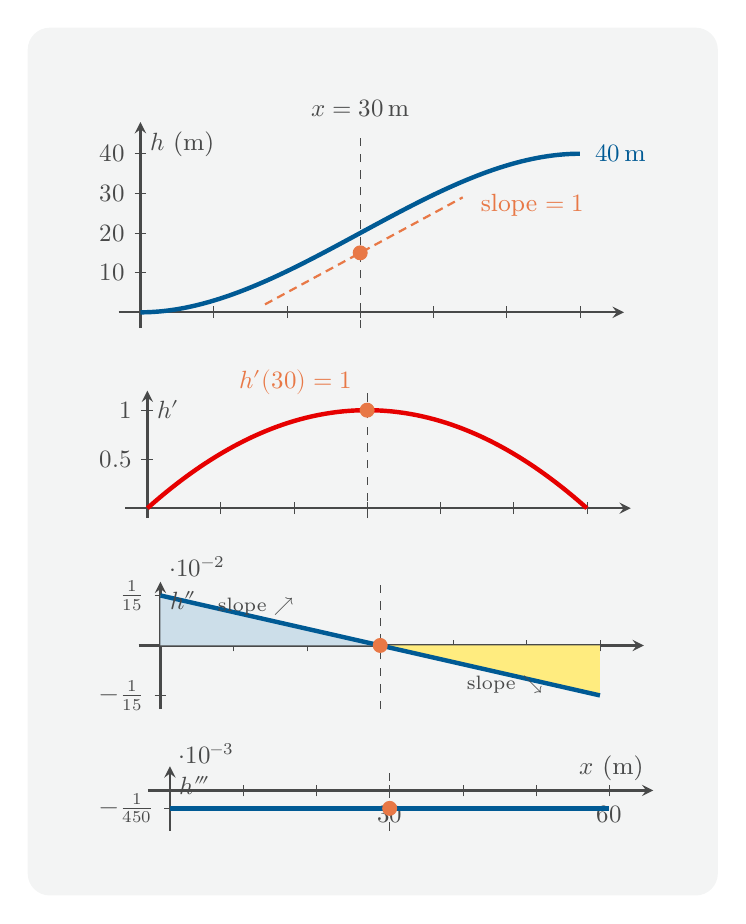
\begin{tikzpicture}[
    show background rectangle,
    background rectangle/.style={fill=my_lightgray, rounded corners=8pt},
    inner frame sep=0.8cm
]

%% ── Shared panel style ────────────────────────────────────────────────────────
%% axis equal is omitted: horizontal unit is metres, vertical units differ
%% across panels (metres, dimensionless slope, m⁻¹, m⁻²).
\pgfplotsset{
    rcpanel/.style={
        width=8cm,
        axis lines=center,
        xmin=-3, xmax=66,
        xtick={0,10,20,30,40,50,60},
        xticklabels={},                         % hidden except on bottom panel
        tick style={color=my_darkgray},
        axis line style={thick, color=my_darkgray},
        ticklabel style={font=\small, color=my_darkgray},
        label style={font=\small, color=my_darkgray},
        clip=false,                             % allow annotations outside frame
    }
}

%% ── Panel 1: h(x) = x²/30 − x³/2700  (height in metres) ────────────────────
\begin{axis}[
    rcpanel,
    name=ax1,
    height=4.2cm,
    ymin=-4, ymax=48,
    ytick={0,10,20,30,40},
    ylabel={$h$~(m)},
]
    %% Height profile
    \addplot[draw=my_darkblue, samples=200, ultra thick, domain=0:60]
        {x^2/30 - x^3/2700};

    %% Tangent at x=30: h(30)=15, h'(30)=1, so y = x−15.  Shown on [17, 44].
    \addplot[draw=my_orange, thick, densely dashed, domain=17:44]
        {x - 15};

    %% Contact point
    \addplot[only marks, mark=*, mark size=2.5pt, color=my_orange]
        coordinates {(30, 15)};

    %% Vertical guide at x=30 linking all four panels
    \draw[dashed, my_darkgray, thin]
        (axis cs:30, -4) -- (axis cs:30, 44);

    %% Label at top of guide
    \node[my_darkgray, font=\small, above=4pt] at (axis cs:30, 44)
        {$x = 30\,\text{m}$};

    %% Tangent-slope annotation
    \node[my_orange, font=\small, right=3pt] at (axis cs:44, 27)
        {slope $= 1$};

    %% Summit label
    \node[my_darkblue, font=\small, right=2pt] at (axis cs:60, 40)
        {$40\,\text{m}$};
\end{axis}

%% ── Panel 2: h'(x) = x(60−x)/900  (dimensionless slope) ────────────────────
\begin{axis}[
    rcpanel,
    name=ax2,
    at={(ax1.outer south west)}, anchor=outer north west,
    yshift=-3mm,
    height=3.2cm,
    ymin=-0.10, ymax=1.20,
    ytick={0, 0.5, 1.0},
    yticklabels={$0$, $0{.}5$, $1$},
    ylabel={$h'$},
]
    \addplot[draw=my_red, samples=200, ultra thick, domain=0:60]
        {x*(60-x)/900};

    %% Maximum slope at x=30
    \addplot[only marks, mark=*, mark size=2.5pt, color=my_orange]
        coordinates {(30, 1)};

    \draw[dashed, my_darkgray, thin]
        (axis cs:30, -0.10) -- (axis cs:30, 1.20);

    \node[my_orange, font=\small, above left=2pt] at (axis cs:30, 1)
        {$h'(30)=1$};
\end{axis}

%% ── Panel 3: h''(x) = (30−x)/450  (rate of slope change) ───────────────────
\begin{axis}[
    rcpanel,
    name=ax3,
    at={(ax2.outer south west)}, anchor=outer north west,
    yshift=-3mm,
    height=3.2cm,
    ymin=-0.085, ymax=0.085,
    ytick={-0.0667, 0, 0.0667},
    yticklabels={$-\tfrac{1}{15}$, $0$, $\tfrac{1}{15}$},
    ylabel={$h''$},
]
    %% Named paths for fill between
    \addplot[draw=none, name path=hddcurve, samples=200, domain=0:60]
        {(30-x)/450};
    \addplot[draw=none, name path=xaxis, domain=0:60]
        {0};

    %% h'' > 0 on [0, 30]: slope is still increasing (light blue)
    \addplot[fill=my_lightblue, draw=none]
        fill between[of=hddcurve and xaxis, soft clip={domain=0:30}];

    %% h'' < 0 on [30, 60]: slope is now decreasing (yellow)
    \addplot[fill=my_yellow, draw=none]
        fill between[of=xaxis and hddcurve, soft clip={domain=30:60}];

    %% Curve drawn on top of fill
    \addplot[draw=my_darkblue, samples=200, ultra thick, domain=0:60]
        {(30-x)/450};

    %% Sign-change point
    \addplot[only marks, mark=*, mark size=2.5pt, color=my_orange]
        coordinates {(30, 0)};

    \draw[dashed, my_darkgray, thin]
        (axis cs:30, -0.085) -- (axis cs:30, 0.085);

    %% Region labels
    \node[my_darkgray, font=\scriptsize] at (axis cs:13,  0.052)
        {slope~$\nearrow$};
    \node[my_darkgray, font=\scriptsize] at (axis cs:47, -0.052)
        {slope~$\searrow$};
\end{axis}

%% ── Panel 4: h'''(x) = −1/450  (constant, cubic structure) ─────────────────
\begin{axis}[
    rcpanel,
    name=ax4,
    at={(ax3.outer south west)}, anchor=outer north west,
    yshift=-3mm,
    height=2.4cm,
    ymin=-0.0050, ymax=0.0030,
    ytick={-0.00222},
    yticklabels={$-\tfrac{1}{450}$},
    xlabel={$x$~(m)},
    xlabel style={font=\small, color=my_darkgray},
    xticklabels={$0$, {}, {}, $30$, {}, {}, $60$},  % labels for 7 ticks
    ylabel={$h'''$},
]
    \addplot[draw=my_darkblue, samples=2, ultra thick, domain=0:60]
        {-1/450};

    \addplot[only marks, mark=*, mark size=2.5pt, color=my_orange]
        coordinates {(30, -1/450)};

    \draw[dashed, my_darkgray, thin]
        (axis cs:30, -0.0050) -- (axis cs:30, 0.0030);
\end{axis}

\end{tikzpicture}
\end{document}
